\section*{Unsupervised relationship mining}

% There are some limitations to modeling sentiment in a supervised way.
%   - Don't have explicit sentiment labels
%   - The interactions between countries is better described
%     by a dimension orthogonal to "war".
%     - Trade
%     - Culture and society

The preceding approach has limitations, however.  Sentiment labels
measure only one kind of interaction: whether countries are at war or
peace; but relationships between countries may be characterized in
many ways, some of which are independent of whether countries are at
war.  For example, the relationship between coutries may be
characterized by trade in goods, or by the exchange of culture and
society. Finally, these labels may be unavailable for a certain period
of time.

% in this section, we will describe a model which will allow us to discover
% unsupervised relationships
%   - We will use a modul much like RTM
%   - RTM is ...
In this section we will describe a model for inferring relationships
between countries in an unsupervised fashion.  This model serves as an
alternative to the model in the last section in that it requires no
explicit labels of the relationship between two different countries.
Instead, it infers a qualitative relationship between countries which
we will interpreted post-hoc.

The significance of this approach is that it infers a relationship
between countries based more on the discussion of these countries than explicit labels.  This will allow us to qualify the discussion of foreign relations.

We will begin by outlining a language model for this purpose.  We will outline the key assumptions of this model -- namely, that a an exposition about two countries comprises language about each country, language about their relationship, and language from some background distribution. We then describe inference for this model, and finally provide an empirical analysis using this model.

\subsection*{A model of unsupervised relationship}
% The assumptions are as follows:
%   - Each country is associated with a background distribution
%   - Each interaction is described by:
%     - words related to either country
%     - miscellaneous words
%     - words about the relationship between the two countries

In the supervised foreign relations discourse model (UFRDM, pronounced
\emph{erf-dum}), our aim is to characterize the relationship between
two countries by inspecting the language used to describe them.  This
model comprises two pieces: a language model for describing the
language used to discuss countries; and a time-series spatial model to
describe the relationship between pairs of countries.  We begin with
the spatial model, which is very similar to the model described in the
last section.

\subsubsection*{Dynamic spatial model}
The assumptions in the unsupervised model are similar to those we used
in the supervised model from the last section.  Each country is
characterized by a position $\bar x_{ct}$ which drifts over time in some
latent space $\mathbb{R^d}$.  Pairs of countries interact according to
the dyadic relationship
\begin{align}
  x_{c_1,d} | \bar x_{c_1,t} & \sim \mathcal{N}(\bar x_{c_1, t}, \sigma_s^2) \\
  x_{c_2,d} | \bar x_{c_2,t} & \sim \mathcal{N}(\bar x_{c_2, t}, \sigma_s^2) \\
  r_{c_1,d} | \bar r_{c_1} & \sim \mathcal{N}(\bar r_{c_1}, \sigma_r^2) \\
  r_{c_2,d} | \bar r_{c_2} & \sim \mathcal{N}(\bar r_{c_2}, \sigma_r^2) \\
  s_d | x_{c_1,d}, x_{c_2,d}, r_{c_1,d}, r_{c_2,d} & = \log( || x_{c_1,d} - x_{c_2,d} ||_2^2 + 1) + r_{c_1} + r_{c_2}), \\
\end{align}
where each country $c$ has an additional intercept $r_c$.
We illustrate this graphically in \myfig{dyadic_chain}.  As before, we
use the extra variables $x$ instead of $\bar x$ for
computational convenience because we can estimate $\bar x$
over time using a Kalman filter.
\begin{figure}
  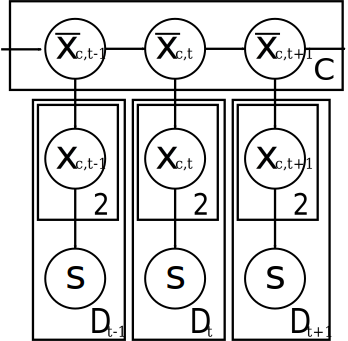
\includegraphics[width=0.3\textwidth]{chapter_foreign_relations/figures/countries_gm_no_text.pdf}
  \caption{The dynamic sentiment model.}
  \label{dyadic_chain}
\end{figure}

\subsubsection*{Binary Relational language model}
We incorporate text using a mixed-membership language model similar to
LDA.  In LDA, each word comes from a specific topic.  In the binary
relational language model, we assume that the words describing a pair
of countries come from topics about those countries.

To be concrete, consider a document discussing Iran and the United
States.  Many words in this document will serve one of
four roles:
\begin{enumerate}
  \item It discusses the U.S.,
  \item It discusses Iran,
  \item It discusses the relationship between the U.S. and Iran. \label{foreign_relations:relationship}
  \item It is a ``filler'' word, providing little contribution to the discussion. \label{foreign_relations:filler}
\end{enumerate}
The first two roles are self-explanatory.  The relationship mentioned
in (\ref{foreign_relations:relationshup}) above could be any type of
relationship -- the goal of this model is of course to discover the
relationships most dominant in a collection of text.  The ``filler''
words mentioned in (\ref{foreign_relations:relationship}) are those
words found in any document -- stopwords, for example -- that are
unrelated to either country or the relationship between them.

We will assume that each document about the United States and Iran is
a mixture of topics. constrain its topics to be exactly that
describe this relationship (providing a single dimension of
flexibility for such words).



We encode these assumptions with
We model this by defining one t $\beta_{C,1}, \ldots, \beta_{C,N_c}$
These ideas are

The full generative model of an interaction is then:
  \begin{algorithm}[tb]
    \begin{algorithmic}
%    \setlength{\topsep}{1pt}
%    \setlength{\itemsep}{2pt}
%    \setlength{\parskip}{1pt}
%    \setlength{\parsep}{1pt}
      %\COMMENT{Generate topics.}
    \FOR{nation $c=1, \ldots, C$}
    \STATE Draw topic $\beta_{\mbox{C},c} \sim \mbox{Dir}(1, \ldots, 1)$.
    \ENDFOR
    \STATE Draw background topic $\beta_{\mbox{B},0} \sim \mbox{Dir}(1, \ldots, 1)$.
    \STATE Draw positive-interaction topic $\beta_{\mbox{S},0} \sim \mbox{Dir}(1, \ldots, 1)$
    \STATE Draw negative-interaction topic $\beta_{\mbox{S},1} \sim \mbox{Dir}(1, \ldots, 1)$
\end{algorithmic}
  \caption{Generate background and interaction topics.}
\end{algorithm}
\begin{algorithm*}
\begin{algorithmic}
    \FOR{document $d=1, \ldots, D$ representing interactions between $c_{d_1},c_{d_2} \in \mathbb{N}$}
    \STATE Draw topic mixture $\theta_d \sim \mbox{Dir}(1, 1, 1, 1)$
    \STATE Define sentiment $\kappa_d = \sigma(s) (2 \sigma{\xi} - 1)$
    \FOR{word $n = 1, \ldots, N_d$}
    \STATE Draw $z_{n} \sim \mbox{Mult}(\theta_d$).
    \IF{$z_n = (1, 0, 0, 0)$}
    \STATE Draw $w_n \sim \beta_{\mbox{C},c_{d_1}}$.
    \ELSIF{$z_n = (0, 1, 0, 0)$}
    \STATE Draw $w_n \sim \beta_{\mbox{C},c_{d_2}}$.
    \ELSIF{$z_n = (0, 0, 1, 0)$}
    \STATE Draw $w_n \sim \beta_{\mbox{B},0}$.
    \ELSIF{$z_n = (0, 0, 0, 1)$}
    \STATE Draw $y_n \sim \mbox{Bin}(\kappa_d)$
    \STATE Draw $w_n \sim \beta_{\mbox{S},y_n}$.
    \ENDIF
    \ENDFOR
    \ENDFOR
  \end{algorithmic}
  \caption{Generate documents given the topics.}
  \label{figure:second_order_algorithm}
%\end{figure}
\end{algorithm*}

\begin{figure}
  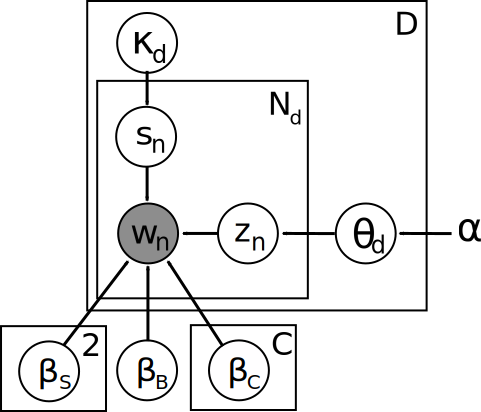
\includegraphics[width=0.4\textwidth]{chapter_foreign_relations/figures/fr_lda_gm.pdf}
  \caption{An unsupervised foreign relations model.  We assign each
    country its own topic $\beta_{C,\cdot}$.  Interactions between
    countries are characterized by the mixture topic
    $\beta_{S,\cdot}$, with an additional background topic $\beta_B$
    to soak up additional noise.}
\end{figure}


\subsubsection*{Empirical analysis}
\paragraph{An economics/military dichotomy}



\begin{table}
%         Country
% 2   united_states
% 3            iran
% 4           japan
% 8          canada
% 13          china
% 17           iraq
% 24        ireland
% 31  great_britain
% 243            X1
%                                                                                             Topics
% 2   officials,military,official,policy,political,support,government,meeting,leaders,administration
% 3                             nuclear,war,program,weapons,officials,arms,oil,hostages,gulf,uranium
% 4               trade,economic,countries,officials,market,economy,world,military,companies,markets
% 8                      trade,country,free,province,border,agreement,speaking,percent,law,officials
% 13               rights,human,trade,relations,officials,nuclear,visit,political,democracy,economic
% 17               forces,weapons,military,troops,officials,government,security,war,chemical,country
% 24                     police,people,province,peace,killed,political,bomb,control,violence,killing
% 31          officials,government,authorities,intelligence,week,people,minister,colony,time,country
% 243             war,political,officials,country,people,military,international,peace,confirmed,week
% mexico: drug,officials,border,law,enforcement,traffickers,agents,police,authorities,trade,cocaine,illegal
  \center
\begin{tabular}{|c|c|}
  \hline
  \textbf{Background topic ($\beta_{B}$)} \\
  \hline
  war \\
  political \\
  officials \\
  country \\
  people \\
  military \\
  international \\
  peace \\
  confirmed \\
  week \\
  following \\
  government \\
  \hline
\end{tabular}
\hspace{30pt} \begin{tabular}{|cc|}
  \hline
  \textbf{Economics topic ($\beta_{S,0}$) vs.} &
  \textbf{Military topic ($\beta_{S,1}$)} \\
  \hline
  million & military \\
  percent & officials \\
  people & soldiers \\
  billion & killed \\
  oil & troops \\
  officials & police \\
  country & forces \\
  money & people \\
  aid & attack \\
  government & border \\
  companies & near \\
  military & air \\
  \hline
\end{tabular}
\\
\vspace{30pt}
\begin{tabular}{|c|c|c|}
  \hline
  \textbf{Pakistan ($\beta_{C,\mbox{\tiny Pakistan}}$)} &
  \textbf{Mexico ($\beta_{C,\mbox{\tiny Mexico}}$)} &
  \textbf{Israel ($\beta_{C,\mbox{\tiny Israel}}$)} \\
% Iran: nuclear,war,program,weapons,officials,arms,oil,hostages,gulf,uranium
% China: rights,human,trade,relations,officials,nuclear,visit,political,democracy,economic
% india: nuclear,countries,border,weapons,tests,talks,nations,military,state,territory,war,militants
% pakistan: nuclear,weapons,military,officials,terrorism,border,war,government,aid,support,countries,militants
% mexico: drug,officials,border,law,enforcement,traffickers,agents,police,authorities,trade,cocaine,illegal
% israel: peace,territories,occupied,talks,officials,negotiations,agreement,state,settlement,security,settlements,violence
  \hline
  nuclear & drug & peace \\
  weapons & officials & territories \\
  military & border & occupied \\
  officials & law & talks \\
  terrorism & enforcement & officials \\
  border & traffickers & negotiations \\
  war & agents & agreement \\
  government & police & state\\
  aid & authorities & settlement \\
  support & trade & security \\
  \hline
\end{tabular}
\vspace{10pt}
\begin{tabular}{|c|c|c|}
  \hline
  \textbf{United States ($\beta_{C,\mbox{\tiny United States}}$)} &
  \textbf{Iran ($\beta_{C,\mbox{\tiny Iran}}$)} &
  \textbf{China ($\beta_{C,\mbox{\tiny China}}$)} \\
% Iran: nuclear,war,program,weapons,officials,arms,oil,hostages,gulf,uranium
% China: rights,human,trade,relations,officials,nuclear,visit,political,democracy,economic
% india: nuclear,countries,border,weapons,tests,talks,nations,military,state,territory,war,militants
% pakistan: nuclear,weapons,military,officials,terrorism,border,war,government,aid,support,countries,militants
% mexico: drug,officials,border,law,enforcement,traffickers,agents,police,authorities,trade,cocaine,illegal
  \hline
  officials & nuclear & rights \\
  military & war & human \\
  official & program & trade \\
  policy & weapons & relations \\
  political & officials & officials \\
  support & arms & nuclear \\
  government & oil & visit \\
  meeting & hostages & political \\
  leaders & gulf & democracy \\
  administration & uranium & economic \\
  \hline
\end{tabular}
\end{table}
\paragraph{National topics}



